\chapter{System Design}
\label{ch:system_design}

\section{Introduction}
This chapter describes the system design of the Seasonal Job Matching Platform Mobile Application. It details the system architecture, state management design, screen navigation flows, PostgreSQL database schemas, API integration, and sequence-based feature interactions. The designs outlined here ensure the system is scalable, secure, and responsive.

\section{System Architecture}
The mobile application uses a hybrid design combining **Clean Architecture** principles with a **Model-View-ViewModel (MVVM)** presentation pattern. This approach separates business rules, data acquisition, and visual elements, allowing each component to be developed and tested independently. Figure~\ref{fig:architecture_layers} shows the architectural layers of the application.

\begin{figure}[htbp]
\centering
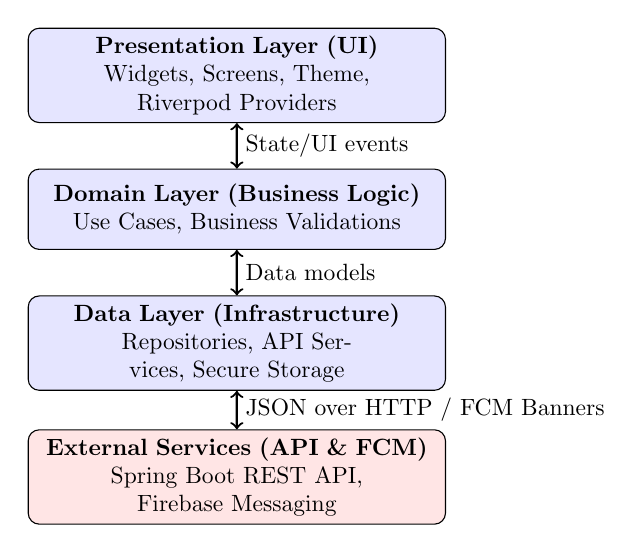
\begin{tikzpicture}[scale=0.85, every node/.style={transform shape}]
    % Define layer styles
    \tikzstyle{layer} = [draw, rectangle, fill=blue!10, text width=6cm, minimum height=1.2cm, align=center, rounded corners]
    \tikzstyle{infra} = [draw, rectangle, fill=red!10, text width=6cm, minimum height=1.2cm, align=center, rounded corners]
    
    % Layer nodes
    \node[layer] (pres) at (0, 6) {\textbf{Presentation Layer (UI)}\\Widgets, Screens, Theme, Riverpod Providers};
    \node[layer] (domain) at (0, 4) {\textbf{Domain Layer (Business Logic)}\\Use Cases, Business Validations};
    \node[layer] (data) at (0, 2) {\textbf{Data Layer (Infrastructure)}\\Repositories, API Services, Secure Storage};
    \node[infra] (external) at (0, 0) {\textbf{External Services (API \& FCM)}\\Spring Boot REST API, Firebase Messaging};
    
    % Direction arrows
    \draw[<->, thick] (pres) -- (domain) node[midway, right] {State/UI events};
    \draw[<->, thick] (domain) -- (data) node[midway, right] {Data models};
    \draw[<->, thick] (data) -- (external) node[midway, right] {JSON over HTTP / FCM Banners};
\end{tikzpicture}
\caption{System Architectural Layering and Dependency Flows}
\label{fig:architecture_layers}
\end{figure}

The system layers are defined as follows:
\begin{itemize}
    \item \textbf{Presentation Layer:} Built using the Flutter framework. It renders the visual widgets, manages UI themes, and coordinates application states using Riverpod providers.
    \item \textbf{Domain Layer:} The logical core of the app. It contains use cases (e.g., \texttt{ApplyForJobUseCase}) that represent specific business logic operations, ensuring they remain independent of data sources and UI widgets.
    \item \textbf{Data Layer:} Coordinates data retrieval and storage. It wraps raw HTTP clients (Dio), implements data repositories (e.g., \texttt{ApplicationsRepository}), and caches credentials securely using \texttt{AuthStorage} (Flutter Secure Storage).
\end{itemize}

\section{MVVM and State Management Design}
State management is governed reactively using the **Flutter Riverpod** framework. The view models are represented by Riverpod's \texttt{Notifier} and \texttt{AsyncNotifier} classes. The UI views listen to these providers and rebuild automatically when the underlying state changes.

Table~\ref{tab:state_management_design} outlines the primary state providers, their structural types, and their cache invalidation lifecycles.

\begin{table}[htbp]
\centering
\caption{State Management Provider Specifications}
\label{tab:state_management_design}
\begin{tabular}{|l|p{4cm}|p{6cm}|}
\hline
\textbf{Provider Reference} & \textbf{Riverpod Provider Type} & \textbf{State Cache Invalidation Lifecycle} \\ \hline
\texttt{authProvider} & \texttt{NotifierProvider} & Retained for the session; cleared on logout or token expiration. \\ \hline
\texttt{personalInformationProvider} & \texttt{AsyncNotifierProvider} & Watches the user's ID; re-fetched when profile fields or favorite lists change. \\ \hline
\texttt{paginatedJobsProvider} & \texttt{AsyncNotifierProvider} & Instantiated on search; resets to page 0 when filters or search terms change. Watches the currency field to trigger invalidation on changes. \\ \hline
\texttt{favoriteJobsProvider} & \texttt{FutureProvider.family} & Invalidated when the user toggles a favorite, triggering a parallel batch fetch. \\ \hline
\texttt{applicationsProvider} & \texttt{AsyncNotifierProvider} & Refreshed immediately on a successful job application. \\ \hline
\texttt{notificationsProvider} & \texttt{FutureProvider.family} & Refreshed when a new FCM token is received or when notifications are marked read. \\ \hline
\texttt{updateStateProvider} & \texttt{NotifierProvider} & Retained for the application session; evaluates version conditions on startup. \\ \hline
\texttt{feedbackProvider} & \texttt{AsyncNotifierProvider} & Transient state handling; resets immediately after feedback submission triggers. \\ \hline
\end{tabular}
\end{table}

\section{Navigation and Screen Flow}
Navigation is implemented using a custom \texttt{NavigationService} containing a global navigator key (\texttt{rootNavigatorKey}). This key allows the application to route pages dynamically without requiring a build context, which is essential for handling global network events (e.g., session timeout routing).

Figure~\ref{fig:screen_flow} shows the navigation flow of the application.

\begin{figure}[htbp]
\centering
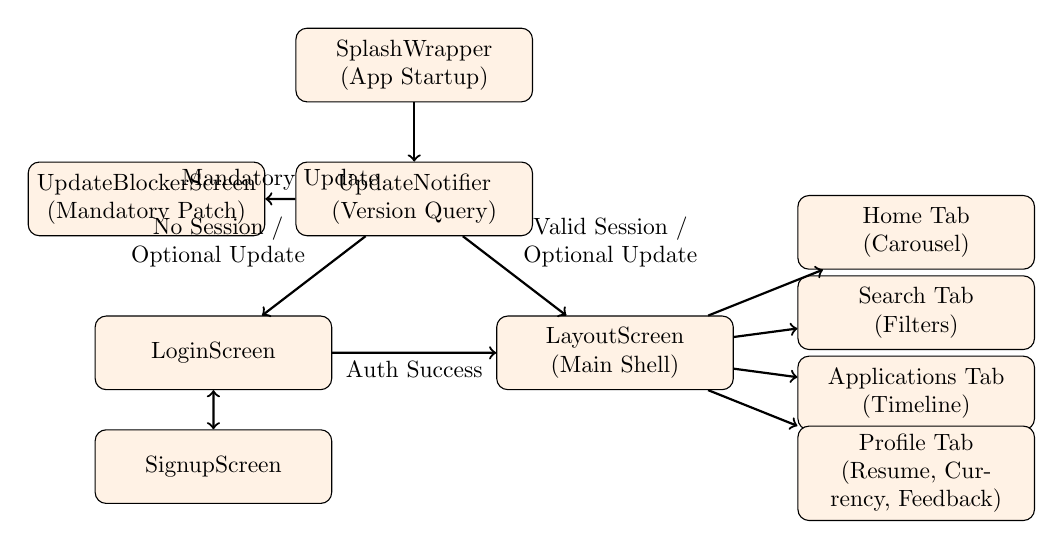
\begin{tikzpicture}[scale=0.85, every node/.style={transform shape}]
    % Define styles
    \tikzstyle{state} = [draw, rectangle, fill=orange!10, text width=3.3cm, minimum height=1.1cm, align=center, rounded corners]
    
    % Nodes
    \node[state] (splash) at (0, 7.8) {SplashWrapper\\(App Startup)};
    \node[state] (update_check) at (0, 5.8) {UpdateNotifier\\(Version Query)};
    \node[state] (blocker) at (-4, 5.8) {UpdateBlockerScreen\\(Mandatory Patch)};
    \node[state] (login) at (-3, 3.5) {LoginScreen};
    \node[state] (signup) at (-3, 1.8) {SignupScreen};
    \node[state] (layout) at (3, 3.5) {LayoutScreen\\(Main Shell)};
    
    \node[state] (home) at (7.5, 5.3) {Home Tab\\(Carousel)};
    \node[state] (search) at (7.5, 4.1) {Search Tab\\(Filters)};
    \node[state] (apps) at (7.5, 2.9) {Applications Tab\\(Timeline)};
    \node[state] (profile) at (7.5, 1.7) {Profile Tab\\(Resume, Currency, Feedback)};
    
    % Flow arrows
    \draw[->, thick] (splash) -- (update_check);
    \draw[->, thick] (update_check) -- node[midway, above] {Mandatory Update} (blocker);
    \draw[->, thick] (update_check) -- node[midway, above left, align=center] {No Session /\\Optional Update} (login);
    \draw[->, thick] (update_check) -- node[midway, above right, align=center] {Valid Session /\\Optional Update} (layout);
    \draw[<->, thick] (login) -- (signup);
    \draw[->, thick] (login) -- node[midway, below] {Auth Success} (layout);
    
    \draw[->, thick] (layout) -- (home);
    \draw[->, thick] (layout) -- (search);
    \draw[->, thick] (layout) -- (apps);
    \draw[->, thick] (layout) -- (profile);
\end{tikzpicture}
\caption{Application Navigation and Screen Flow with Update Checking}
\label{fig:screen_flow}
\end{figure}

On app startup, the \texttt{SplashWrapper} checks if a valid JWT token exists in the device's secure storage. If it is missing or expired, the user is routed to the \texttt{LoginScreen}; otherwise, the user is directed to the main \texttt{LayoutScreen}, which hosts the tab bar.

\section{Database Design (PostgreSQL Schema)}
The backend database is structured in PostgreSQL. The tables are designed to support fast indexing on key queries, such as retrieving job listings by category, checking applications by user, or retrieving notification histories.

Figure~\ref{fig:er_diagram} shows the database schema and entity relationships.

\begin{figure}[htbp]
\centering
\begin{tikzpicture}[scale=0.8, every node/.style={transform shape}]
    % Define table style
    \tikzstyle{table} = [draw, rectangle, fill=yellow!15, text width=4cm, align=left, rounded corners, minimum height=2.5cm]
    
    % Table nodes
    \node[table] (users) at (0, 5) {
        \textbf{users}\\
        \hline
        PK: id (INT)\\
        name (VARCHAR)\\
        email (VARCHAR, UNIQUE)\\
        phone (VARCHAR)\\
        country (VARCHAR)\\
        fields\_of\_interest (JSONB)
    };
    
    \node[table] (resumes) at (-5, 5) {
        \textbf{resumes}\\
        \hline
        PK: id (INT)\\
        FK: user\_id (INT)\\
        education (JSONB)\\
        experience (JSONB)\\
        skills (JSONB)
    };
    
    \node[table] (jobs) at (5, 0) {
        \textbf{jobs}\\
        \hline
        PK: id (INT)\\
        title (VARCHAR)\\
        company (VARCHAR)\\
        location (VARCHAR)\\
        type (VARCHAR)\\
        salary (NUMERIC)\\
        status (VARCHAR)
    };
    
    \node[table] (applications) at (0, 0) {
        \textbf{applications}\\
        \hline
        PK: id (INT)\\
        FK: user\_id (INT)\\
        FK: job\_id (INT)\\
        describe\_yourself (TEXT)\\
        status (VARCHAR)\\
        created\_at (TIMESTAMP)
    };
    
    \node[table] (notifications) at (-5, 0) {
        \textbf{notifications}\\
        \hline
        PK: id (INT)\\
        FK: user\_id (INT)\\
        title (VARCHAR)\\
        body (TEXT)\\
        is\_read (BOOLEAN)\\
        created\_at (TIMESTAMP)
    };

    % Connections showing cardinality
    \draw[-, thick] (users) -- (resumes) node[midway, above] {1:1};
    \draw[-, thick] (users) -- (applications) node[midway, right] {1:N};
    \draw[-, thick] (jobs) -- (applications) node[midway, above] {1:N};
    \draw[-, thick] (users) -- (notifications) node[midway, above] {1:N};
\end{tikzpicture}
\caption{Entity-Relationship (ER) Database Schema}
\label{fig:er_diagram}
\end{figure}

The database schema enforces the following rules and relationships:
\begin{itemize}
    \item \textbf{Users and Resumes (1:1 Relationship):} A user has exactly one professional resume. Resume entries (skills, experience, and education) are stored as flexible PostgreSQL \texttt{JSONB} arrays to accommodate variable section formats.
    \item \textbf{Users and Applications (1:N Relationship):} An applicant can submit multiple job applications, but each application belongs to one user.
    \item \textbf{Jobs and Applications (1:N Relationship):} A job listing can receive multiple applications, but each application points to one listing.
\end{itemize}

\section{API Integration and Endpoints}
The client communicates with the Spring Boot backend REST service. Responses are parsed into type-safe Dart models generated using the Freezed package.

Table~\ref{tab:api_endpoints} outlines the primary API endpoints integrated into the mobile app services layer.

\begin{table}[htbp]
\centering
\caption{API Endpoint Mapping and Services Summary}
\label{tab:api_endpoints}
\begin{tabular}{|l|p{2cm}|p{4.5cm}|p{4cm}|}
\hline
\textbf{Endpoint Path} & \textbf{HTTP Verb} & \textbf{Payload / Query parameters} & \textbf{Service Caller Class} \\ \hline
\texttt{/api/users/login} & POST & Email, Password & \texttt{AuthService} \\ \hline
\texttt{/api/users} & POST & Signup details JSON & \texttt{AuthService} \\ \hline
\texttt{/api/users/\{uid\}} & PATCH & \texttt{name}, \texttt{email}, \texttt{number}, \texttt{country}, or \texttt{currency} & \texttt{PersonalInformationService} \\ \hline
\texttt{/api/jobs} & GET & \texttt{page}, \texttt{size} & \texttt{JobsServicesProvider} \\ \hline
\texttt{/api/jobs/filter} & GET / POST & \texttt{query}, \texttt{type}, \texttt{location}, \texttt{minSalary} & \texttt{JobsServicesProvider} \\ \hline
\texttt{/api/applications/user/\{uid\}/job/\{jid\}} & POST & \texttt{describeYourself} & \texttt{ApplicationsRepository} \\ \hline
\texttt{/api/users/\{uid\}/favorite-jobs} & PATCH & Favorite job IDs array & \texttt{PersonalInformationService} \\ \hline
\texttt{/api/resumes/\{id\}} & PATCH & \texttt{skillsToAdd}, \texttt{skillsToRemove} (Diff arrays) & \texttt{ResumeService} \\ \hline
\texttt{/api/notifications/\{uid\}} & GET & None & \texttt{NotificationsApiService} \\ \hline
\texttt{/api/feedback} & POST & \texttt{title}, \texttt{body}, \texttt{userEmail} (optional) & \texttt{FeedbackService} \\ \hline
\texttt{/repos/\{owner\}/\{repo\}/releases/latest} & GET & None (GitHub Release API) & \texttt{UpdateNotifier} \\ \hline
\end{tabular}
\end{table}

\section{Sequence and Interaction Flows}
This section illustrates the sequence of interactions between the user interface, the local state controllers, the networking layer, and the backend services for two core application workflows.

\subsection{Authentication Flow and Token Registration}
The login process validates user credentials, caches the returned JWT token, and registers the device's Firebase token. Figure~\ref{fig:seq_auth} shows the sequence diagram for this flow.

\begin{figure}[htbp]
\centering
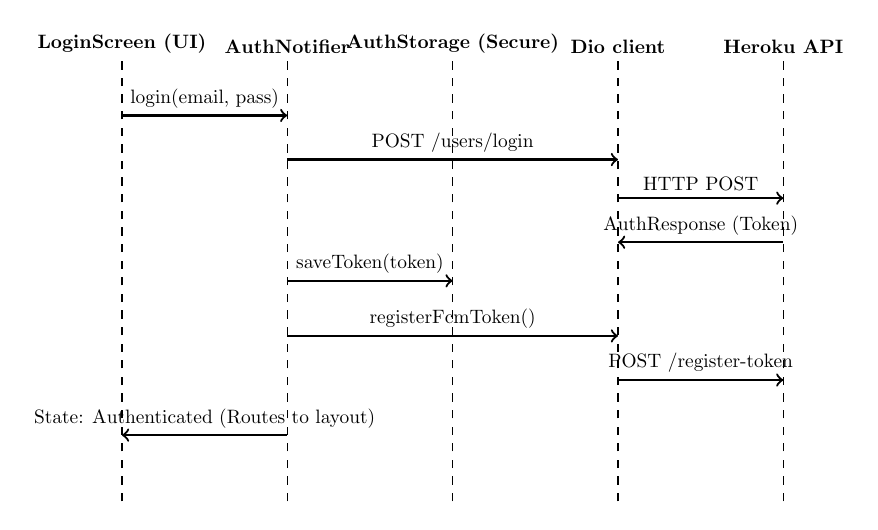
\begin{tikzpicture}[scale=0.7, every node/.style={transform shape}]
    % Vertical Lifelines
    \draw[dashed] (0, 0) -- (0, 8) node[above] {\textbf{LoginScreen (UI)}};
    \draw[dashed] (3, 0) -- (3, 8) node[above] {\textbf{AuthNotifier}};
    \draw[dashed] (6, 0) -- (6, 8) node[above] {\textbf{AuthStorage (Secure)}};
    \draw[dashed] (9, 0) -- (9, 8) node[above] {\textbf{Dio client}};
    \draw[dashed] (12, 0) -- (12, 8) node[above] {\textbf{Heroku API}};

    % Messages
    \draw[->, thick] (0, 7) -- (3, 7) node[midway, above] {login(email, pass)};
    \draw[->, thick] (3, 6.2) -- (9, 6.2) node[midway, above] {POST /users/login};
    \draw[->, thick] (9, 5.5) -- (12, 5.5) node[midway, above] {HTTP POST};
    \draw[<-, thick] (9, 4.7) -- (12, 4.7) node[midway, above] {AuthResponse (Token)};
    \draw[->, thick] (3, 4) -- (6, 4) node[midway, above] {saveToken(token)};
    \draw[->, thick] (3, 3) -- (9, 3) node[midway, above] {registerFcmToken()};
    \draw[->, thick] (9, 2.2) -- (12, 2.2) node[midway, above] {POST /register-token};
    \draw[<-, thick] (0, 1.2) -- (3, 1.2) node[midway, above] {State: Authenticated (Routes to layout)};
\end{tikzpicture}
\caption{Authentication and Secure Registration Sequence Diagram}
\label{fig:seq_auth}
\end{figure}

\subsection{Job Application Submission and Cache Update}
To prevent duplicate job applications, the app uses an optimistic UI state coupled with backend validation. Figure~\ref{fig:seq_apply} shows the sequence diagram for this flow.

\begin{figure}[htbp]
\centering
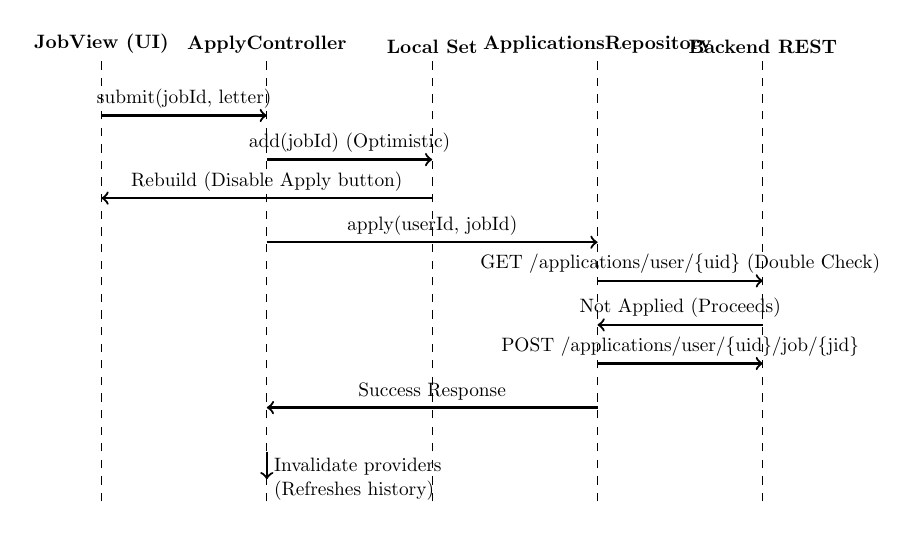
\begin{tikzpicture}[scale=0.7, every node/.style={transform shape}]
    % Vertical Lifelines
    \draw[dashed] (0, 0) -- (0, 8) node[above] {\textbf{JobView (UI)}};
    \draw[dashed] (3, 0) -- (3, 8) node[above] {\textbf{ApplyController}};
    \draw[dashed] (6, 0) -- (6, 8) node[above] {\textbf{Local Set}};
    \draw[dashed] (9, 0) -- (9, 8) node[above] {\textbf{ApplicationsRepository}};
    \draw[dashed] (12, 0) -- (12, 8) node[above] {\textbf{Backend REST}};

    % Messages
    \draw[->, thick] (0, 7) -- (3, 7) node[midway, above] {submit(jobId, letter)};
    \draw[->, thick] (3, 6.2) -- (6, 6.2) node[midway, above] {add(jobId) (Optimistic)};
    \draw[<-, thick] (0, 5.5) -- (6, 5.5) node[midway, above] {Rebuild (Disable Apply button)};
    \draw[->, thick] (3, 4.7) -- (9, 4.7) node[midway, above] {apply(userId, jobId)};
    \draw[->, thick] (9, 4.0) -- (12, 4.0) node[midway, above] {GET /applications/user/\{uid\} (Double Check)};
    \draw[<-, thick] (9, 3.2) -- (12, 3.2) node[midway, above] {Not Applied (Proceeds)};
    \draw[->, thick] (9, 2.5) -- (12, 2.5) node[midway, above] {POST /applications/user/\{uid\}/job/\{jid\}};
    \draw[<-, thick] (3, 1.7) -- (9, 1.7) node[midway, above] {Success Response};
    \draw[->, thick] (3, 0.9) -- (3, 0.4) node[right, align=left] {Invalidate providers\\(Refreshes history)};
\end{tikzpicture}
\caption{Optimistic Job Application and Double-Submission Prevention Sequence}
\label{fig:seq_apply}
\end{figure}

\subsection{Over-the-Air Update Check and Update Enforcement}
The system validates the application version at startup, fetching version descriptors from GitHub and locking the interface if a mandatory patch is active. Figure~\ref{fig:seq_ota} outlines this sequence.

\begin{figure}[htbp]
\centering
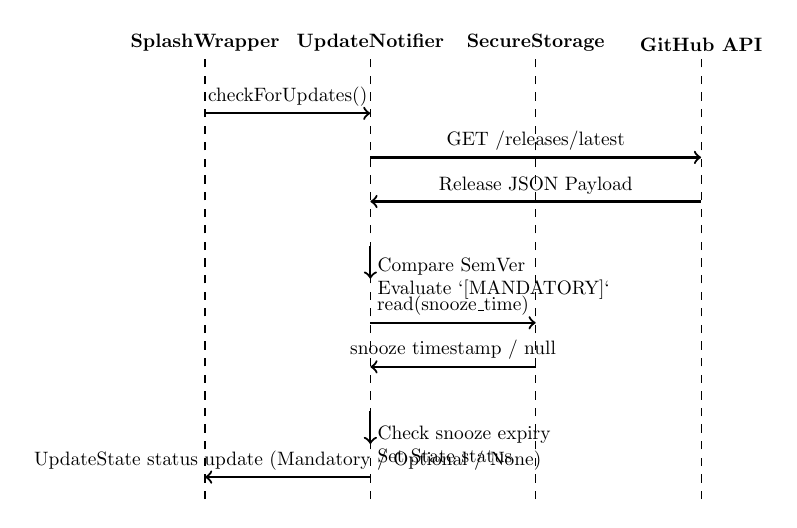
\begin{tikzpicture}[scale=0.7, every node/.style={transform shape}]
    % Vertical Lifelines
    \draw[dashed] (0, 0) -- (0, 8) node[above] {\textbf{SplashWrapper}};
    \draw[dashed] (3, 0) -- (3, 8) node[above] {\textbf{UpdateNotifier}};
    \draw[dashed] (6, 0) -- (6, 8) node[above] {\textbf{SecureStorage}};
    \draw[dashed] (9, 0) -- (9, 8) node[above] {\textbf{GitHub API}};

    % Messages
    \draw[->, thick] (0, 7) -- (3, 7) node[midway, above] {checkForUpdates()};
    \draw[->, thick] (3, 6.2) -- (9, 6.2) node[midway, above] {GET /releases/latest};
    \draw[<-, thick] (3, 5.4) -- (9, 5.4) node[midway, above] {Release JSON Payload};
    \draw[->, thick] (3, 4.6) -- (3, 4.0) node[right, align=left] {Compare SemVer\\Evaluate `[MANDATORY]`};
    
    % Branching choice: Optional vs Mandatory
    \draw[->, thick] (3, 3.2) -- (6, 3.2) node[midway, above] {read(snooze\_time)};
    \draw[<-, thick] (3, 2.4) -- (6, 2.4) node[midway, above] {snooze timestamp / null};
    \draw[->, thick] (3, 1.6) -- (3, 1.0) node[right, align=left] {Check snooze expiry\\Set State status};
    \draw[<-, thick] (0, 0.4) -- (3, 0.4) node[midway, above] {UpdateState status update (Mandatory / Optional / None)};
\end{tikzpicture}
\caption{Startup OTA Update Verification and Blocker Sequence Diagram}
\label{fig:seq_ota}
\end{figure}

\subsection{Issue Reporting and Feedback Submission}
The feedback channel processes bug descriptions, checking anonymous toggles and resolving emails locally before sending requests. Figure~\ref{fig:seq_feedback} describes the sequence.

\begin{figure}[htbp]
\centering
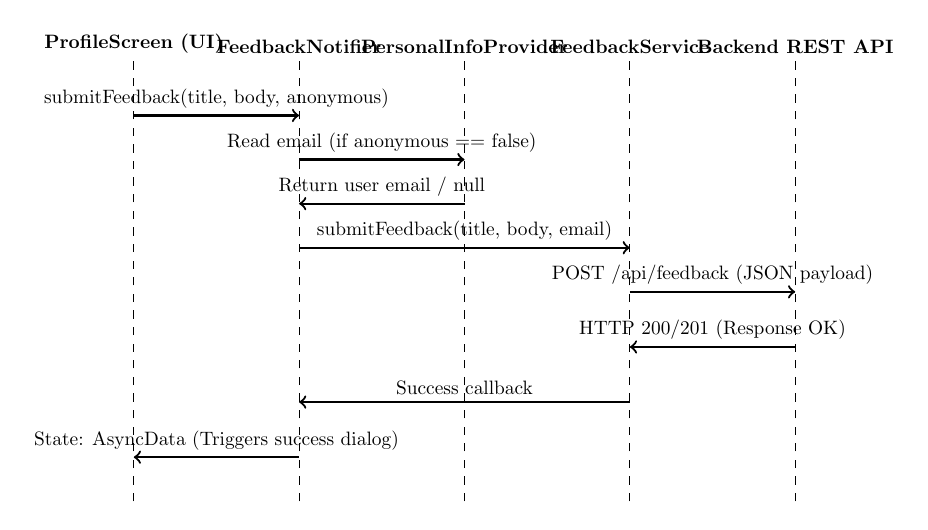
\begin{tikzpicture}[scale=0.7, every node/.style={transform shape}]
    % Vertical Lifelines
    \draw[dashed] (0, 0) -- (0, 8) node[above] {\textbf{ProfileScreen (UI)}};
    \draw[dashed] (3, 0) -- (3, 8) node[above] {\textbf{FeedbackNotifier}};
    \draw[dashed] (6, 0) -- (6, 8) node[above] {\textbf{PersonalInfoProvider}};
    \draw[dashed] (9, 0) -- (9, 8) node[above] {\textbf{FeedbackService}};
    \draw[dashed] (12, 0) -- (12, 8) node[above] {\textbf{Backend REST API}};

    % Messages
    \draw[->, thick] (0, 7) -- (3, 7) node[midway, above] {submitFeedback(title, body, anonymous)};
    \draw[->, thick] (3, 6.2) -- (6, 6.2) node[midway, above] {Read email (if anonymous == false)};
    \draw[<-, thick] (3, 5.4) -- (6, 5.4) node[midway, above] {Return user email / null};
    \draw[->, thick] (3, 4.6) -- (9, 4.6) node[midway, above] {submitFeedback(title, body, email)};
    \draw[->, thick] (9, 3.8) -- (12, 3.8) node[midway, above] {POST /api/feedback (JSON payload)};
    \draw[<-, thick] (9, 2.8) -- (12, 2.8) node[midway, above] {HTTP 200/201 (Response OK)};
    \draw[<-, thick] (3, 1.8) -- (9, 1.8) node[midway, above] {Success callback};
    \draw[<-, thick] (0, 0.8) -- (3, 0.8) node[midway, above] {State: AsyncData (Triggers success dialog)};
\end{tikzpicture}
\caption{Issue Reporting and Feedback Submission Sequence Diagram}
\label{fig:seq_feedback}
\end{figure}
